\documentclass[10pt]{article}
\usepackage[final]{pdfpages}
\usepackage{cleveref}
\usepackage{xparse}
\usepackage{hyperref}
\usepackage{geometry}
\usepackage{amsmath}
\usepackage{graphicx}
\usepackage{caption}
\usepackage{subcaption}
\usepackage[section]{placeins}
\usepackage{listings}
\usepackage{verbatim}
%\usepackage{harvard}
\usepackage[dcucite,abbr]{harvard}
\usepackage{sectsty}
\usepackage{html}
\usepackage{url}
\sectionfont{\rmfamily\mdseries\Large}
\subsectionfont{\rmfamily\mdseries\itshape\large}

\geometry{
  %body={6.5in, 8.5in},
  left=2.5cm,
  right=2cm,
  top=2cm,
  bottom=2cm
}

\linespread{1.213}
\begin{document}
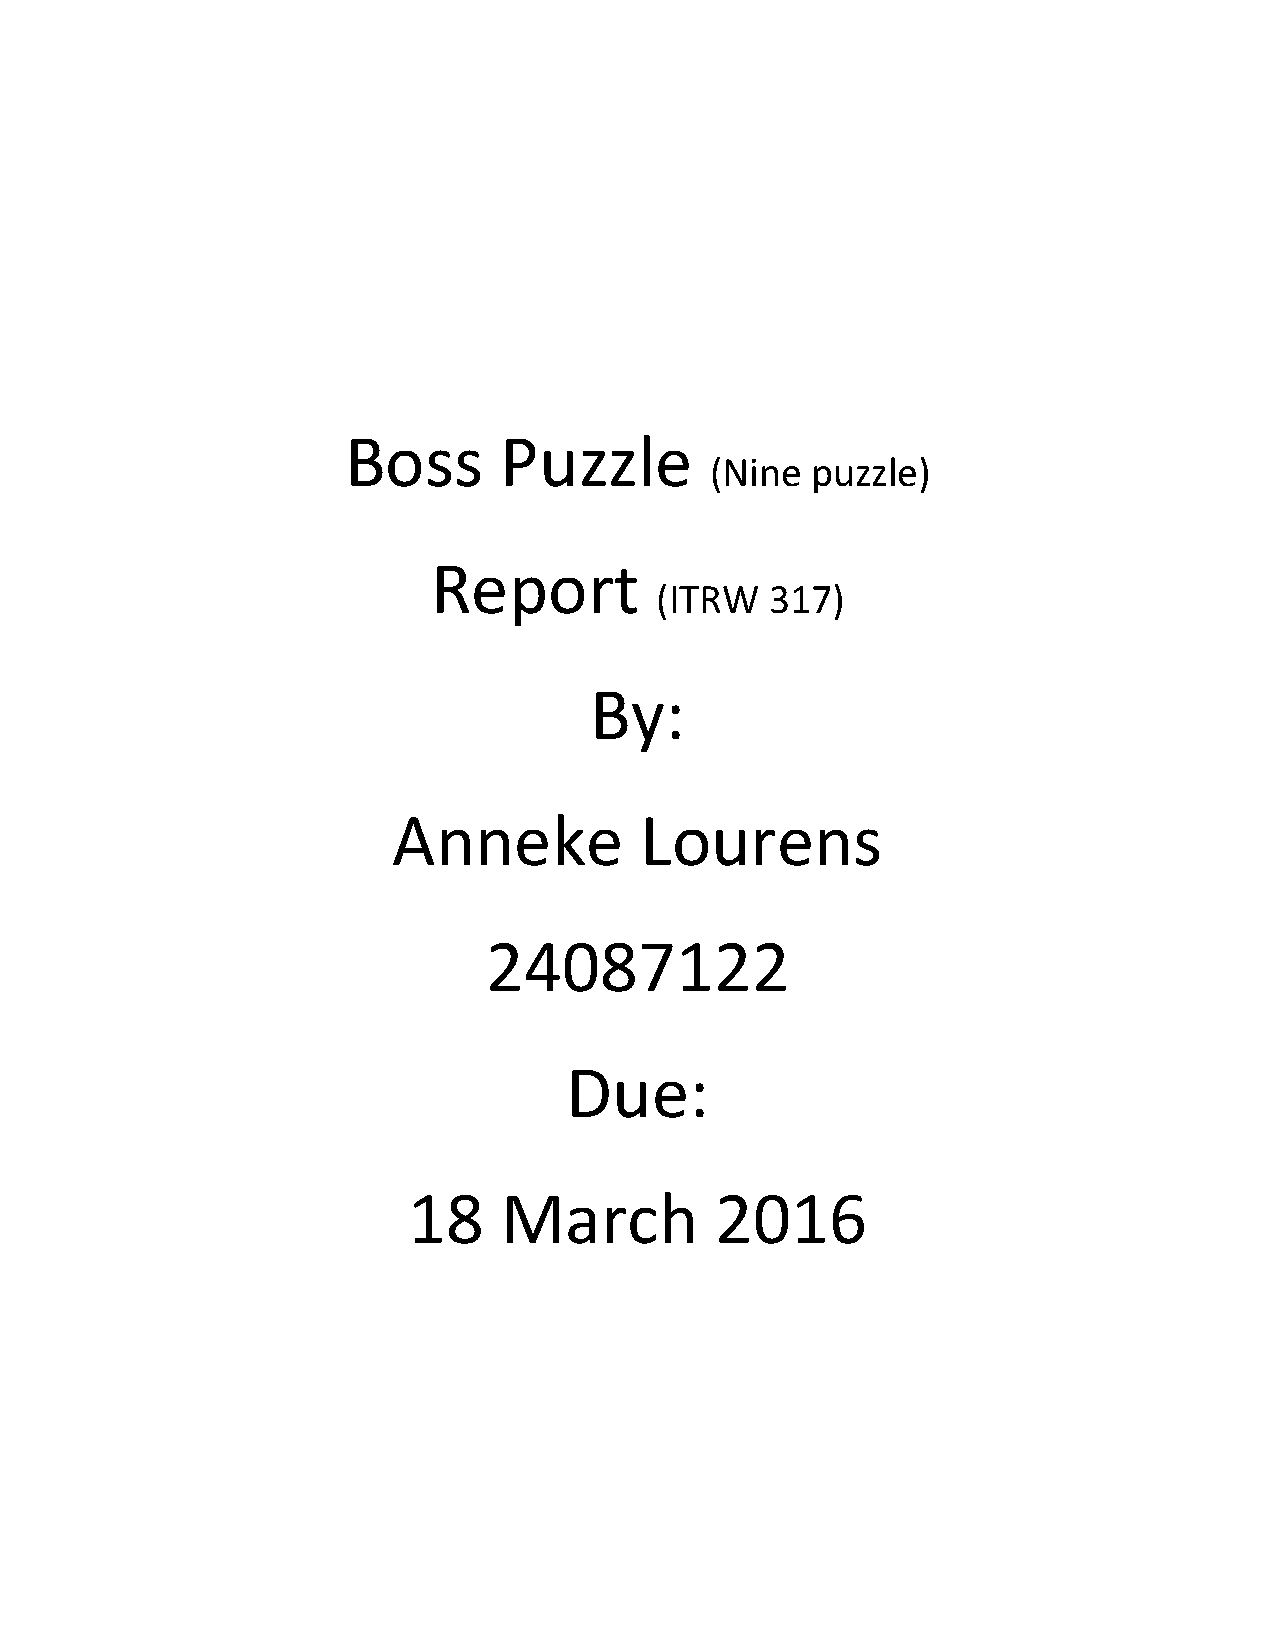
\includepdf{./BossPuzzle.pdf}
\newpage
index
\newpage
\section{Introduction}
This report is about the Nine-Puzzle.  The document will give a little bit of background information and also where did the nine puzzle has started.  This report will also include how to play the game. A step by step guide is included that tell you how to set up the puzzle and how to run the Nine-puzzle game that is included in the folder.

\section{Literature Study}
\subsection{Background and History}
The objective of the 9-puzzle is to move the tiles in the given 3X3 board to make a picture complete or to give the solution (Reinefeld).
\section{User Guide}
\subsection{How to make a .csv file}
Step 1:
\\Open the file named "waarde\_puzzle.csv" in Notepad$++$ or Notepad.
Remember that the file must have "," in between the numbers and there must only be 8 numbers and a lowercase b where the blank space in the puzzle must be (Figure~\ref{csv}).
Figure~\ref{waardes} is an example of what the .csv file looks in notepad$++$ or Notepad. The first row is the puzzle that is presented to the player and the second row is the solved puzzle.  If the player has saved its puzzle to continue later there will be a third row in the .csv file that shows the moves that the player has made already.
\begin{figure}
\centering
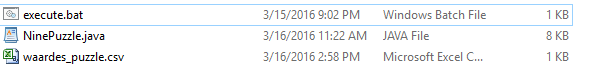
\includegraphics[scale=0.7]{./Prente/csv.png}
\caption{This is the files that one get which will run the nine puzzle}
\label{csv}
\end{figure}
\begin{figure}
\centering
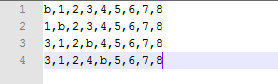
\includegraphics[scale=1]{./Prente/waardes.png}
\caption{How the data looks in the .csv file.  This data will be used in the nine puzzle.}
\label{waardes}
\end{figure}
\subsection{How to begin the Nine-puzzle}
Step 1:
\\If you have your own .csv file - right click on the execute.bat file and open it with notepad.
Change the filename of the .csv file.  Save the file and exit it.  Double-click on the execute.bat file to run the program. Figure~\ref{csv}
\\Step 2:
\begin{figure*}[b!]
    \centering
    \begin{subfigure}[b]{0.5\textwidth}
        \centering
        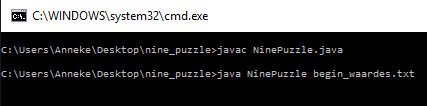
\includegraphics[scale=0.8]{./Prente/begincmd.png}
        \caption{If you have run the execute.bat file this lines will show in the CMD }
        \label{begincmd}
    \end{subfigure}%
 
    \begin{subfigure}[b]{0.5\textwidth}
        \centering
        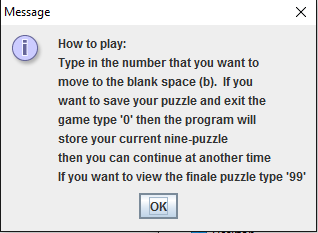
\includegraphics[scale=0.8]{./Prente/MessageBegin.png}
        \caption{The program will show this message directly after you have run the execute.bat file}
        \label{MessageBegin}
    \end{subfigure}
    \caption{\label{1}}
   \end{figure*}
\\If the program has run you will see Figure~\ref{1}
\\Step 3: 
\\Enter a "y" for you are a new player or "n" for you are not a new player Figure~\ref{prent1}
\begin{figure}
\centering
 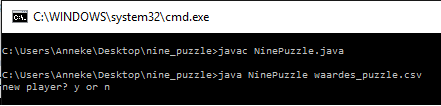
\includegraphics[scale=0.8]{./Prente/prent1.png}
  \caption{You will be asked if you are a new player or not}
  \label{prent1}
\end{figure}
\\Step 4:
\begin{figure}
\centering
 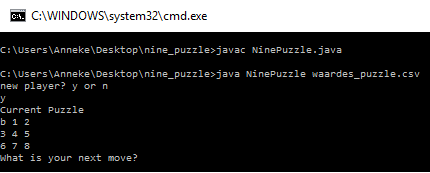
\includegraphics[scale=0.8]{./Prente/prent2.png}
 \caption{After specifying that you are a new player or not the program will give the begin puzzle}
 \label{prent2}
\end{figure}
\\After step 3 is completed the begin puzzle will be given. Figure~\ref{prent2}
\\Step 5:
\begin{figure}
\centering
 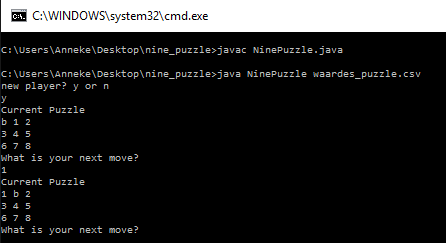
\includegraphics[scale=0.8]{./Prente/prent3.png}
 \caption{After a move is made}
 \label{prent3}
\end{figure}
\\Enter the number that you want to move like in Figure~\ref{prent3}. The game will move that number to the blank space(b) and give the updated puzzle again.
\subsection{Functionality}
How to stop, save and exit the program:
\\If you want to stop playing and play again later then you can type "0" then the puzzle will be saved and the game will exit Figure~\ref{2}.
\begin{figure*}[b!]
    \centering
    \begin{subfigure}[b]{0.5\textwidth}
        \centering
        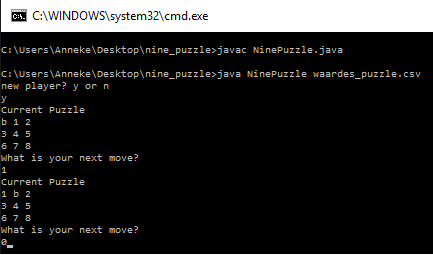
\includegraphics[scale=0.8]{./Prente/prent4.png}
        \caption{If you type in 0}
        \label{prent4}
    \end{subfigure}%
 
    \begin{subfigure}[b]{0.5\textwidth}
        \centering
        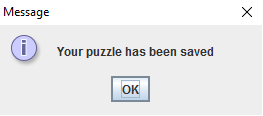
\includegraphics[scale=0.8]{./Prente/prent5.png}
        \caption{The message will show that your puzzle has been saved}
        \label{prent5}
    \end{subfigure}
    \caption{\label{2}}
   \end{figure*}
   
If you have won the game, the program will save your work and show a message to congratulate you and show how many moves you have made to solve the puzzle Figure~\ref{prent6}.
\begin{figure}
\centering
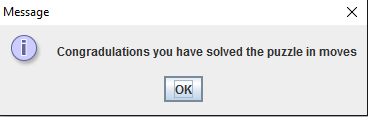
\includegraphics[scale=0.8]{./Prente/prent6.png}
\caption{The congratulation message}
\label{prent6}
\end{figure}

If you want to view the finale puzzle you type in 99 Figure~\ref{prent7}.
\begin{figure}
\centering
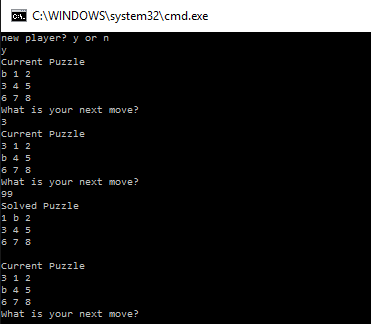
\includegraphics[scale=0.8]{./Prente/prent7.png}
\caption{Solved puzzle is shown in the program}
\label{prent7}
\end{figure}

\section{Code}
 \begin{tiny}
 \lstinputlisting[language=java, firstline=1, lastline=222]{./NinePuzzle.java}
   \end{tiny}
   \section{Bibliography}
   Reinefeld, A.Complete Solution of the Eight-Puzzle and the Bene t of Node Ordering in IDA*.
   \url{http://www.laborion.com/Portals/0/Ai/Heuristicssearch/93ijcai.pdf} Date of access: 8 Maart 2016.
\bibliographystyle{dcu} 
\bibliography{harvard}%where the bib file must be read
\end{document}